\subsubsection{Listar}

  \paragraph{}Para mostrar esta lista, es necesario establecer el asesor para
  el que mostrar los cursos académicos disponibles. Para ello, habrá que elegir
  el asesor en la lista desplegable que se muestra en la figura
  \ref{capturaPantallaSelectAsesor}.

  \begin{figure}[!ht]
    \begin{center}
      \fbox{
      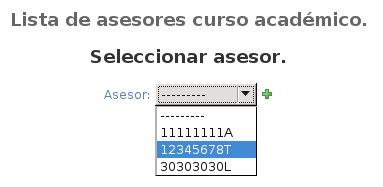
\includegraphics[scale=0.55]{4.Funcionamiento_Aplicacion/4.3.Gestion/4.3.1.Administrador_Principal/4.3.1.10.AsesorCA/select_asesor.png}
      }
      \caption{Captura de pantalla de la lista desplegable para seleccionar asesor para el usuario \textit{Administrador principal}.}
      \label{capturaPantallaSelectAsesor}
    \end{center}
  \end{figure}

  \paragraph{}Nótese que si no existieran elementos disponibles en el sistema,
  la lista desplegable aparecería vacía. Por tanto, se proporciona al usuario
  un icono, representado por una cruz verde, para añadir nuevos elementos al
  sistema. Este icono es el mostrado en la figura \ref{capturaBotonAdd}. Al
  pulsar dicho botón, aparecerá la ventana de creación de un nuevo elemento.

  \paragraph{}Una vez seleccionado el asesor entre los disponibles, se muestra
  la lista completa de asesores curso académico que aparecen en el sistema. La
  figura \ref{capturaPantallaListaAsesoresCAAdminPrincipal} muestra una captura
  de pantalla de la lista de asesores curso académico.

  \begin{figure}[!ht]
    \begin{center}
      \fbox{
      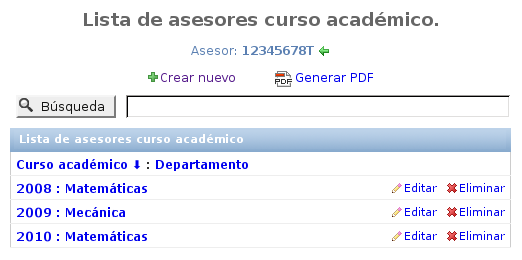
\includegraphics[scale=0.55]{4.Funcionamiento_Aplicacion/4.3.Gestion/4.3.1.Administrador_Principal/4.3.1.10.AsesorCA/lista_asesoresCA.png}
      }
      \caption{Captura de pantalla de la lista de asesores curso académico para el usuario \textit{Administrador principal}.}
      \label{capturaPantallaListaAsesoresCAAdminPrincipal}
    \end{center}
  \end{figure}
